% Native TikZ redraw: 2008 新课标文(海南,宁夏) Q17 图1
% Source: inputs/original_01.pdf p1 Q17; inputs/2008_new_curriculum_liberal_q17_fig1.png
% Exact construction: A(0,0), B(2,0), C(1,1); ACD equilateral outside AC; E = AC ∩ DB.
\usetikzlibrary{calc}
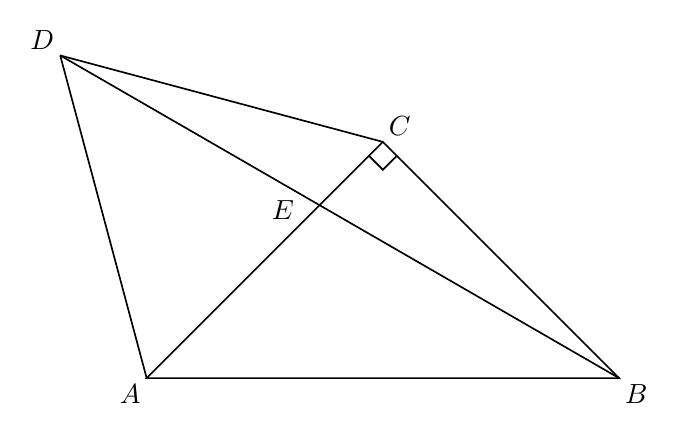
\begin{tikzpicture}[x=1cm,y=1cm,font=\normalsize,
  geometry edge/.style={solid,line width=.6pt},
  geometry mark/.style={solid,line width=.6pt},
  geometry label/.style={font=\normalsize,inner sep=1pt}]
\coordinate (A) at (0,0);
\coordinate (B) at (6,0);
\coordinate (C) at (3,3);
\coordinate (D) at (-1.09808,4.09808);
\coordinate (E) at (2.19615,2.19615);
\draw[geometry edge] (A)--(B)--(C)--cycle;
\draw[geometry edge] (A)--(D);
\draw[geometry edge] (C)--(D);
\draw[geometry edge] (D)--(B);
\coordinate (R1) at ($(C)!.25cm!(A)$);
\coordinate (R2) at ($(C)!.25cm!(B)$);
\coordinate (R3) at ($(R1)+(R2)-(C)$);
\draw[geometry mark] (R1)--(R3)--(R2);
\node[geometry label,below left=1pt] at (A) {$A$};
\node[geometry label,below right=1pt] at (B) {$B$};
\node[geometry label,above right=1pt] at (C) {$C$};
\node[geometry label,above left=1pt] at (D) {$D$};
\node[geometry label] at (1.73,2.135) {$E$};
\end{tikzpicture}
